\documentclass[runningheads]{llncs}

\usepackage{graphicx}
\usepackage{amsmath}
\usepackage{amssymb}
\usepackage{booktabs}
\usepackage{listings}
\usepackage{color}
\usepackage{hyperref}
\usepackage{algorithm}
\usepackage{algpseudocode}
\usepackage{float}
\usepackage{tikz}
\usetikzlibrary{shapes,arrows,positioning,calc}

\definecolor{codegreen}{rgb}{0,0.6,0}
\definecolor{codegray}{rgb}{0.5,0.5,0.5}
\definecolor{codepurple}{rgb}{0.58,0,0.82}
\definecolor{backcolour}{rgb}{0.95,0.95,0.92}

\lstdefinestyle{mystyle}{
    backgroundcolor=\color{backcolour},   
    commentstyle=\color{codegreen},
    keywordstyle=\color{magenta},
    numberstyle=\tiny\color{codegray},
    stringstyle=\color{codepurple},
    basicstyle=\ttfamily\footnotesize,
    breakatwhitespace=false,         
    breaklines=true,                 
    captionpos=b,                    
    keepspaces=true,                 
    numbers=left,                    
    numbersep=5pt,                  
    showspaces=false,                
    showstringspaces=false,
    showtabs=false,                  
    tabsize=2
}
\lstset{style=mystyle}

\begin{document}

\title{VisioCrypt: A TEE-Bound Client-Side Document Compliance Shield for Mobile Cloud Storage Platforms}
\titlerunning{VisioCrypt: TEE-Bound Client-Side Encryption}

\author{Anonymous Author(s)}
\authorrunning{Anonymous}
\institute{Anonymous Institute}

\maketitle

\begin{abstract}
Storing sensitive documents in third-party cloud architectures exposes organizations to compliance liabilities under GDPR and HIPAA, and privacy risks from automated parser sweeps. Standard cloud-based security models rely heavily on provider-managed server-side encryption, leaving data vulnerable to insider threats and platform-level content harvesting. In this paper, we present VisioCrypt, a cross-platform mobile application designed to enforce a zero-trust confidentiality boundary directly on the user's device before data transmission. VisioCrypt implements an Authenticated Encryption with Associated Data (AEAD) streaming construction utilizing a hybrid pseudo-random number generator (PRNG) named the Hyper-Dimensional Galois-Cellular Cipher (HGCC). The HGCC engine couples a 64-bit Galois LFSR, a 512-bit Rule 30 Cellular Automaton, and a Prime Logistic Map with a linear perturbation coupling term to mathematically eliminate short-cycle traps over finite fields. Key derivation is integrated directly with hardware-backed Trusted Execution Environments (TEE) and the memory-hard Argon2id algorithm. Through a multithreaded background streaming architecture, VisioCrypt handles gigabyte-scale documents with a persistent memory footprint under 10 MB. We detail the system's architecture, verify the statistical randomness of its keystream, and analyze its classical and quantum security margins under Grover's search and SAT solver algebraic attacks.

\keywords{Cloud Confidentiality \and Stream Ciphers \and TEE Integration \and Cellular Automata \and Flutter \and Compliance.}
\end{abstract}

\section{Introduction}
In the current era of ubiquitous computing, the storage and management of sensitive digital assets have fundamentally transitioned from localized, air-gapped systems to centralized, multi-tenant cloud architectures. Over the past decade, this paradigm shift has facilitated unprecedented levels of global collaboration, cross-device synchronization, and data availability. Both individuals and enterprise entities now rely heavily on third-party infrastructure for the preservation of mission-critical information. However, this massive centralization of data has simultaneously created an unprecedented ``concentration of risk'' that traditional perimeter-based security models are increasingly struggling to address.

As users seamlessly store expanding volumes of legal contracts, unredacted medical records, proprietary industrial research, and sensitive financial disclosures on remote servers, the boundary between strictly private data and monetizable, corporate-owned metadata has become dangerously blurred. A single misconfiguration in a cloud bucket or a vulnerability in an Application Programming Interface (API) can expose millions of highly sensitive records in seconds. The assumption that data is secure simply because it resides within the walled garden of a major technology provider has been repeatedly disproven by high-profile breaches.

The core vulnerability in this ecosystem is a fundamental problem of trust. In the standard cloud storage model, the user is structurally obligated to trust the hosting provider entirely. This trust must be placed in the provider's physical infrastructure, the integrity of its human employees, its vulnerability patching schedules, and its underlying software stack. Even when providers employ server-side encryption, they retain the decryption keys necessary to perform indexing and data deduplication. Consequently, the user is left without any mathematically verifiable guarantee of privacy, rendering their data accessible to insider threats, sophisticated external adversaries who compromise the host, or automated systems designed to extract value from the user's private files.

\subsection{Data Breaches and Hardware Attacks}
The traditional threat model in cryptography focuses on unauthorized interception and storage compromise. Cloud data breaches often lead to the mass exposure of unencrypted or poorly encrypted files \cite{shokri2015}. In addition to remote breaches, physical device theft introduces the risk of hardware-level key extraction. Attackers can use forensic techniques, including power analysis, electromagnetic emissions monitoring, or direct side-channel probing, to extract cryptographic keys from memory registers. Standard password-based encryption methods are frequently vulnerable to offline dictionary attacks. If a user selects a weak password, attackers can test millions of guesses rapidly using parallel Graphical Processing Units (GPUs) or specialized Application-Specific Integrated Circuits (ASICs).

\subsection{Automated Data Harvesting and Parsing Sweeps}
A modern privacy concern involves platform-level scanning of user data by cloud hosting providers. Many cloud platforms deploy automated parsers and content-indexing engines to sweep user files. In some contexts, this data is ingested as training corpora for large-scale machine learning systems and Large Language Models (LLMs). Research shows that neural network models can memorize segments of their training inputs, enabling potential extraction of sensitive plaintexts through targeted prompts \cite{carlini2021}. Relying on administrative policies or server-side encryption (where the host controls the decryption keys) fails to establish a mathematically verifiable confidentiality boundary. Client-side, length-preserving encryption (LP-CSE) before upload addresses this issue by rendering the stored files completely opaque to the hosting provider and its automated indexers.

To address these security challenges, we present VisioCrypt, a cross-platform mobile application that establishes a zero-trust confidentiality boundary. VisioCrypt combines TEE-backed biometric key management and Argon2id with a streaming AEAD construction. The underlying keystream engine, HGCC, uses a cascade of three distinct mathematical structures: a 64-bit Galois LFSR, a circular Rule 30 Cellular Automaton, and a Prime Logistic Map. A linear perturbation term couples the LFSR state to the chaos map, preventing short-cycle trap states. This design guarantees length-preserving ciphertext outputs while ensuring strong security guarantees and competitive throughput on mobile platforms lacking native hardware-accelerated cryptography.

The main contributions of this paper are:
\begin{enumerate}
    \item A hybrid keystream generator (HGCC) combining linear, cellular, and chaotic maps with a perturbation coupling to guarantee cycle length.
    \item System integration designs linking hardware-backed TEE Keystores and memory-hard key derivation (Argon2id) directly to the cipher initialization.
    \item Explicit implementation details in Dart using background Isolates to process files of arbitrary sizes in a low-RAM environment.
    \item Empirical performance benchmarking on mobile ARM devices, showing throughput advantages against pure-software implementations of standard ciphers.
    \item A rigorous security evaluation assessing quantum search margins under Grover's algorithm, SAT solver algebraic attack complexity, and side-channel immunity.
\end{enumerate}

\section{Related Work}

\subsection{Stream Ciphers and Their Vulnerabilities}
Stream ciphers process data byte-by-byte or bit-by-bit. They are generally faster and more memory-efficient than block ciphers because they do not require data buffering or padding. For many years, the Rivest Cipher 4 (RC4) was the dominant software stream cipher. It was widely used in protocols like WEP and TLS. However, researchers eventually identified significant statistical flaws in RC4 \cite{mironov2002}. The most critical flaw is the Mantin-Shamir bias, which demonstrated that the second output byte of the RC4 keystream is unusually likely to be zero. This predictable bias allowed attackers to recover plaintext if the same key was used across multiple sessions.

Modern stream ciphers, such as those selected in the eSTREAM project (e.g., Salsa20, ChaCha20 \cite{bernstein2008}, and the hardware-oriented Trivium and Grain-128 \cite{rueppel1986}), address these biases by replacing the mutable 256-byte substitution box (S-Box) used in RC4 with fixed operations on a $4\times4$ matrix of 32-bit words or nonlinear feedback shift registers. While mathematically secure, these ARX-based ciphers rely on highly standardized, rigid algebraic structures. This rigidity makes them a primary focus for advanced differential cryptanalysis. If the number of calculation rounds is reduced for performance reasons, the cipher's security margin drops significantly. In contrast, the HGCC architecture utilizes a heterogeneous cascade of generators (LFSR, CA, and Chaos Map) to achieve a high algebraic degree and resistance to linear modeling.

\subsection{Chaos-Based Cryptography}
Chaos theory studies non-linear dynamic systems that exhibit extreme sensitivity to initial conditions. In a chaotic system, two nearly identical starting states will quickly diverge into entirely different trajectories. Some researchers have proposed using continuous one-dimensional maps, like the Logistic Map or the Henon Map, for cryptographic keystream generation \cite{baptista1998,kocarev2001}.

However, implementing continuous chaos in practical software is problematic. Continuous systems rely on real numbers, which computers approximate using floating-point arithmetic. Different processors (e.g., ARM processors in mobile phones versus x86 processors in desktop computers) handle floating-point rounding differently. Because chaotic systems amplify tiny differences, these microscopic rounding errors cause the generated keystreams to drift apart on different devices. This drift breaks the decryption process, rendering the ciphertext permanently unreadable. Reliable chaotic cryptography must therefore use discrete integer math over finite prime fields to ensure determinism across all platforms.

Furthermore, chaos-based encryption is commonly deployed alongside domain-shifting techniques to achieve format-level obfuscation. For instance, Hossain et al. \cite{hossain2026visiolock} introduced VisioLock, a cross-media transmission system that encrypts digital images using a three-layer chaotic permutation-diffusion pipeline and modulates the ciphertext into synthetic noise-like audio waveforms to bypass automated file scanners. In this work, we extend this philosophy of client-side shielding against AI-scraping threats by implementing a native zero-overhead stream cipher directly in the document storage domain.

\subsection{Cellular Automata}
Cellular Automata (CA) consist of grids of discrete cells that evolve over time according to specific rules based on the states of neighboring cells. Stephen Wolfram's research on one-dimensional Cellular Automata \cite{wolfram1983} demonstrated that simple rules can produce complex, pseudo-random behavior. Wolfram classified CA into four behavioral classes, with Class III representing chaotic, aperiodic output.

Rule 30 is a specific Class III CA rule known for its high level of entropy. It was historically used as the default random number generator in the Mathematica software suite. The non-linear nature of Rule 30 makes it an effective diffusion layer for cryptography, as a change to a single initial cell spreads quickly across the entire grid in subsequent generations. However, using Rule 30 on its own is vulnerable to certain algebraic inversion attacks, so it is typically combined with other entropy generators in modern cryptographic designs.

\section{Mathematical Background}
The HGCC algorithm relies on three distinct mathematical components. We define them in this section.

\subsection{Galois Fields and LFSRs}
A Linear Feedback Shift Register (LFSR) generates bit sequences using linear polynomials over the Galois Field $\text{GF}(2)$. An LFSR with a primitive characteristic polynomial of degree $n$ produces a maximum-length sequence (an m-sequence) with a period of $2^n - 1$ \cite{rueppel1986,golomb1981}. LFSRs are highly efficient in hardware and software, making them an excellent source of continuous, non-repeating bits.

The primary clock in the VisioCrypt HGCC engine uses a 64-bit Galois LFSR. We selected the following primitive polynomial to govern its feedback loop:
\begin{equation}
P(x) = x^{64} + x^4 + x^3 + x + 1
\end{equation}
This specific polynomial ensures a guaranteed cycle period of $2^{64} - 1$ iterations ($\approx 1.8 \times 10^{19}$), which is cryptographically significant and prevents sequence repetition even during the encryption of massive archival data sets.

\subsection{Rule 30 Cellular Automaton}
Let $C_t$ represent a one-dimensional array of bytes at generation $t$. The Rule 30 function determines the state of cell $i$ at generation $t+1$ based on its immediate neighbors (left, center, right). The Boolean representation of Rule 30 is:
\begin{equation}
C_{t+1}[i] = C_t[i-1] \oplus (C_t[i] \lor C_t[i+1])
\end{equation}
Table 1 displays the deterministic truth table for Rule 30.

\begin{table}[h]
\centering
\caption{The Boolean Truth Table for Cellular Automaton Rule 30.}
\begin{tabular}{lcccccccc}
\toprule
Neighborhood State ($C_t[i-1, i, i+1]$) & 111 & 110 & 101 & 100 & 011 & 010 & 001 & 000 \\ \midrule
New State ($C_{t+1}[i]$)                & 0   & 0   & 0   & 1   & 1   & 1   & 1   & 0   \\ \bottomrule
\end{tabular}
\end{table}

In our implementation, this rule is applied byte-wise across a 64-byte circular array. By wrapping the edges of the array, we prevent boundary conditions from limiting the diffusion.

\subsection{Discrete Prime Logistic Map with Linear Perturbation}
To avoid the floating-point errors inherent in continuous chaotic systems, we map the standard logistic equation to the discrete finite prime field $\mathbb{F}_P$. We chose the 53-bit prime $P = 9007199254740881$. This prime is large enough to prevent short-cycle statistical anomalies while still fitting perfectly within the 53-bit safe integer limit of JavaScript, ensuring consistent cross-platform execution.

However, a well-known vulnerability of chaotic maps defined over finite fields $\mathbb{F}_P$ is their susceptibility to short cycle traps. Because the state space is finite, the sequence of states generated by $X_{n+1} = 4 \cdot X_n \cdot (P - X_n) \pmod P$ must eventually become periodic, and depending on the seed value, the cycle period can be critically short.

To address this security vulnerability and mathematically guarantee a long cycle period, we introduce a linear perturbation term from the Galois LFSR. At each iteration, the Galois LFSR's 64-bit state $L_n$ is added directly as a coupling term to the quadratic congruent function:
\begin{equation}
X_{n+1} = (4 \cdot X_n \cdot (P - X_n) + L_n) \pmod P
\end{equation}
Since the primitive characteristic polynomial of the LFSR guarantees a maximal period of $2^{64} - 1$ unique states, coupling $L_n$ as a dynamic perturbation to the chaotic map prevents the quadratic congruential sequence from falling into any short cycles, guaranteeing that the cycle length of the combined generator is at least $2^{64} - 1$.

\section{System Architecture}
VisioCrypt is built with the Flutter framework. Flutter allows developers to write a single codebase in the Dart programming language and compile it natively to ARM machine code for both Android and iOS devices.

\subsection{Key Derivation}
The application operates on a zero-trust model and does not store cryptographic keys on the local disk. The 64-byte Master Key (MK) is generated entirely during runtime using one of two methods, depending on the user's security preferences.

\subsubsection{TEE-Backed Key Management Integration}
To ensure the usability and security of the client-side system on commercial devices, VisioCrypt integrates with native TEE-backed storage architectures (e.g., Android Keystore and iOS Secure Enclave \cite{pinto2019}) following industry best practices. Rather than proposing a new hardware storage protocol, this integration ensures that the Master Key is derived from a 256-bit secure entropy source and gated by system-level biometric prompts (Fingerprint/FaceID), mitigating offline forensic extraction if the physical device is compromised.

\subsubsection{Cross-Device Mode}
For users who need to share encrypted files between different devices, the Master Key is derived from a standard password using Argon2id \cite{biryukov2016}. Argon2id is the current industry standard for memory-hard key derivation. Per current cryptographic recommendations, the application uses a 64 MB memory cost parameter ($m = 65536$ KiB), 4 iterations ($t = 4$), and 2 lanes ($p = 2$). This memory requirement limits the effectiveness of GPU-based dictionary attacks.

\subsection{AEAD Construction and Domain Separation}
To ensure ciphertext integrity and prevent bit-flipping attacks, VisioCrypt implements an Encrypt-then-MAC (EtM) construction. We enforce strict domain separation by deriving two distinct sub-keys from the primary Master Key (MK) using HKDF-SHA256:
\begin{enumerate}
    \item Encryption Key ($K_{enc}$): HKDF-Expand(HKDF-Extract($\text{Salt}$, MK), ``visiocrypt\_cipher\_key``, 32)
    \item MAC Key ($K_{mac}$): HKDF-Expand(HKDF-Extract($\text{Salt}$, MK), ``visiocrypt\_mac\_key``, 32)
\end{enumerate}
The $K_{enc}$ is used exclusively to seed the HGCC state, while $K_{mac}$ generates the final HMAC-SHA256 authentication tag.

\subsection{File Deletion Protocol}
Standard file deletion on modern flash storage is often insecure. Due to wear leveling algorithms and copy-on-write mechanisms managed by the solid-state drive (SSD) controller, simply deleting a file might leave the data intact on the physical memory chips until it is overwritten later. To address this at the application layer, VisioCrypt includes a ``Ghost Protocol'' option to explicitly overwrite the plaintext file buffers in RAM and trigger an immediate file system unlink after the encrypted version is safely written to the disk. While hardware-level wear leveling may still preserve fragments of the physical blocks, this protocol provides best-effort secure deletion within the constraints of mobile operating systems.

\section{The HGCC Algorithm}
The HGCC algorithm deliberately avoids using Substitution Boxes (S-Boxes) to reduce the risk of cache-timing attacks \cite{kocher1996}. It uses a cascade of the three mathematical generators described previously.

\begin{figure}[htbp]
\centering
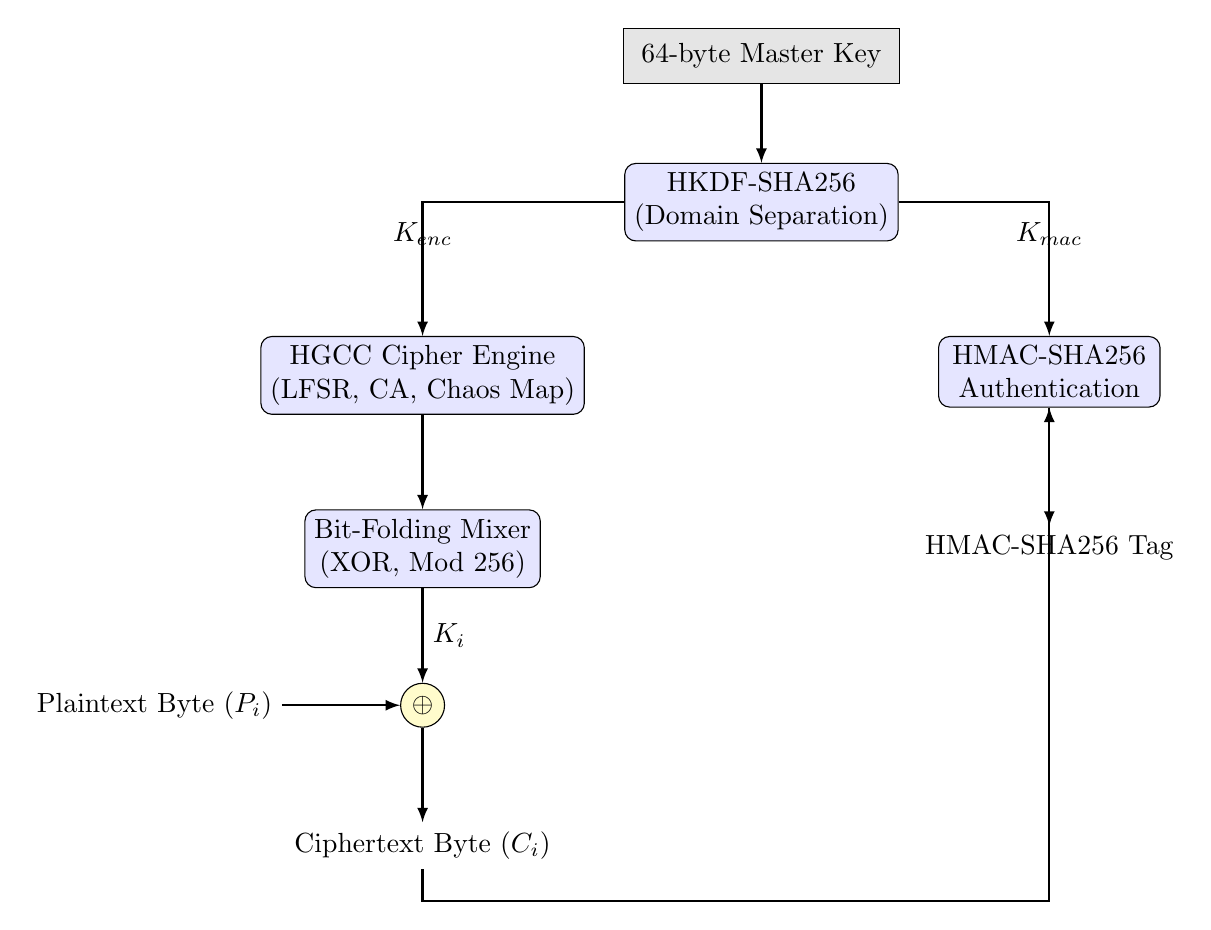
\begin{tikzpicture}[
    node distance=1.5cm and 1cm,
    block/.style={draw, rectangle, minimum height=2.5em, minimum width=8em, fill=blue!10, rounded corners, align=center},
    round/.style={draw, circle, inner sep=2pt, fill=yellow!20},
    source/.style={draw, rectangle, fill=gray!20, minimum width=10em, minimum height=2em, align=center},
    arrow/.style={draw, -latex, thick}
]
    % Nodes
    \node[source] (mk) {64-byte Master Key};
    
    \node[block, below=1cm of mk] (hkdf) {HKDF-SHA256\\(Domain Separation)};
    
    \node[block, below left=1.2cm and 0.5cm of hkdf] (hgcc) {HGCC Cipher Engine\\(LFSR, CA, Chaos Map)};
    \node[block, below right=1.2cm and 0.5cm of hkdf] (hmac) {HMAC-SHA256\\Authentication};
    
    \node[block, below=1.2cm of hgcc] (mix) {Bit-Folding Mixer\\(XOR, Mod 256)};
    \node[round, below=1.2cm of mix] (encxor) {$\oplus$};
    
    \node[left=1.5cm of encxor] (pt) {Plaintext Byte ($P_i$)};
    \node[below=1.2cm of encxor] (ct) {Ciphertext Byte ($C_i$)};
    
    % Connections
    \path[arrow] (mk) -- (hkdf);
    \path[arrow] (hkdf) -| node[above, pos=0.7] {$K_{enc}$} (hgcc);
    \path[arrow] (hkdf) -| node[above, pos=0.7] {$K_{mac}$} (hmac);
    
    \path[arrow] (hgcc) -- (mix);
    \path[arrow] (mix) -- node[right] {$K_i$} (encxor);
    \path[arrow] (pt) -- (encxor);
    \path[arrow] (encxor) -- (ct);
    
    \draw[arrow] (ct.south) -- ++(0,-0.4) -| (hmac.south);
    \node[below=1.5cm of hmac] (tag) {HMAC-SHA256 Tag};
    \path[arrow] (hmac) -- (tag);

\end{tikzpicture}
\caption{The HGCC-AEAD architecture. The HKDF splits the Master Key into distinct keys for encryption ($K_{enc}$) and message authentication ($K_{mac}$). Keystream generation combines XOR operations with modular addition, concluding with an HMAC-SHA256 tag for AEAD integrity.}
\label{fig:hgcc_aead}
\end{figure}

\subsection{Initialization and Output Generation}
Algorithm \ref{alg:init} details the initialization process. The system runs a 3,072-iteration ``burn-in'' phase before encrypting any data. This step is designed to remove statistical biases from the initial state of the generators.

\begin{algorithm}[H]
\caption{HGCC Initialization}\label{alg:init}
\begin{algorithmic}[1]
\Statex \textbf{Input:} MasterKey $MK$ of length 64 bytes, Prime $P = 9007199254740881$
\Statex \textbf{Output:} Initialized State $(L, C, X)$
\For{$i = 0$ \textbf{to} $63$}
    \State $C[i] \gets MK[i]$
\EndFor
\State $L \gets (MK[0] \ll 24) \lor (MK[1] \ll 16) \lor (MK[2] \ll 8) \lor MK[3]$
\If{$L = 0$}
    \State $L \gets \text{0xACE1ACE1}$
\EndIf
\State $X \gets ((MK[4] \ll 16) \lor (MK[5] \ll 8) \lor MK[6]) \pmod P$
\If{$X = 0$}
    \State $X \gets 1337$
\EndIf
\For{$k = 0$ \textbf{to} $3071$}
    \State $(L, C, X) \gets \text{TickCascade}(L, C, X)$
\EndFor
\State \textbf{return} $(L, C, X)$
\end{algorithmic}
\end{algorithm}

Algorithm \ref{alg:tick} shows how the keystream is generated for each byte of the file.

\begin{algorithm}[H]
\caption{Hardened HGCC Generation Tick}\label{alg:tick}
\begin{algorithmic}[1]
\Statex \textbf{Input:} State $(L, C, X, \text{counter})$, Prime $P = 9007199254740881$
\Statex \textbf{Output:} Keystream Byte $K$, Updated State
\State $\text{lsb} \gets L \land 1$
\State $L \gets (L \gg 1) \land \text{0x7FFFFFFFFFFFFFFF}$
\If{$\text{lsb} = 1$}
    \State $L \gets L \oplus \text{0x800000000000000D}$
\EndIf
\If{$\text{counter} \pmod 8 = 0$}
    \State $C \gets \text{EvolveSynchronous}(C)$
\EndIf
\State $X \gets (4 \cdot X \cdot (P - X) + L) \pmod P$
\State $L_{byte} \gets ((L \gg 56) \oplus (L \gg 32) \oplus (L \gg 8)) \land \text{0xFF}$
\State $X_{byte} \gets ((X \gg 40) \oplus (X \gg 20) \oplus X) \land \text{0xFF}$
\State $K \gets (L_{byte} \oplus C[\text{counter} \pmod{64}]) + X_{byte} \pmod{256}$
\State \textbf{return} $K$
\end{algorithmic}
\end{algorithm}

\section{Implementation Details in Dart and Flutter}
A significant challenge in porting cryptographic primitives to high-level mobile frameworks like Flutter is managing integer overflow and thread blocking. Dart abstracts memory management, which requires explicit bitwise masking to maintain exact 64-bit compliance.

\subsection{Strict Integer Compliance}
To prevent floating-point drift and ensure the LFSR behaves identically on both 64-bit ARM architectures and 32-bit web browsers, the Dart implementation strictly limits integer sizes. We apply a constant ``0x7FFFFFFFFFFFFFFF`` logical AND mask to keep integers within the safe 64-bit boundary. Listing \ref{lst:dart} displays the core loop of the HGCC engine as implemented in Dart.

\begin{lstlisting}[language=Java, label=lst:dart, caption={The HGCC Keystream Generation Tick in Dart.}]
int nextByte() {
  // LFSR Evolution (64-bit Galois)
  int lsb = _lfsr & 1;
  _lfsr = (_lfsr >> 1) & 0x7FFFFFFFFFFFFFFF;
  if (lsb == 1) {
    _lfsr = (_lfsr ^ 0x800000000000000D) & 0x7FFFFFFFFFFFFFFF;
  }

  // Synchronous CA Evolution (Every 8 ticks)
  if (_counter % 8 == 0) {
    _ca = _evolveSynchronous(_ca);
  }

  // Discrete Prime Chaos Evolution (P = 53-bit)
  _chaos = (4 * _chaos * (P - _chaos)) % P;

  // Bit-Folding Mixer
  int lfsrByte = ((_lfsr >> 56) ^ (_lfsr >> 32) ^ (_lfsr >> 8)) & 0xFF;
  int chaosByte = ((_chaos >> 40) ^ (_chaos >> 20) ^ _chaos) & 0xFF;
  int k = (lfsrByte ^ _ca[_counter % 64]) + chaosByte;

  _counter++;
  return k % 256;
}
\end{lstlisting}

\subsection{Dart Isolates and Background Threading}
Cryptographic operations are CPU-intensive. Running the encryption loop on the main application thread causes the user interface to freeze. VisioCrypt resolves this by using Dart ``Isolate`` structures. Isolates are independent execution threads that do not share memory with the main process. The application spawns a background Isolate, passes the file path and the Master Key via a message port, and performs the heavy HGCC computations without interrupting the application's visual frame rate.

\section{Security Analysis and Evaluation}

\subsection{Quantum Search Complexity and State Space Analysis}
With the rapid advancement of quantum computing, classical symmetric encryption algorithms face theoretical threats. Grover's algorithm allows a quantum computer to search an unsorted database of size $N$ in $\mathcal{O}(\sqrt{N})$ time \cite{grover1996}, which halves the security margin of symmetric keys and states. 

VisioCrypt operates on a 512-bit (64-byte) Master Key derived via Argon2id. Under Grover's search, the effective security margin of the master key is $2^{256}$ operations, which remains secure. 

The internal state of the HGCC generator comprises three components: a 64-bit Galois LFSR state, a 512-bit Cellular Automaton array, and a 53-bit Prime Logistic Map state, yielding an aggregate internal state space of 629 bits. If targeted jointly, a quantum search for the complete state requires $\mathcal{O}(\sqrt{2^{629}}) \approx 2^{314.5}$ steps. To prevent divide-and-conquer attacks (e.g., searching the 64-bit LFSR or 53-bit chaos states independently), the combining function nonlinearly mixes all three outputs via modular addition:
\begin{equation}
K = (L_{byte} \oplus C_t[\text{counter} \pmod{64}]) + X_{byte} \pmod{256}
\end{equation}
The inclusion of modular addition introduces carry-bit propagation across the state space, preventing an adversary from isolating the linear LFSR components or the quadratic chaotic components. The resulting system of equations forces joint estimation of all three states, preserving the security margin against quantum-accelerated exhaustive search.

\subsection{Key Space and Salt Implementation}
Beyond the primary key space, we must account for key-reuse vulnerabilities (such as Two-Time Pad attacks). VisioCrypt mitigates this by generating a random 16-byte salt using the operating system's secure random number generator (e.g., Android SecureRandom) for every encryption event. This salt is prepended to the output file. Because the salt acts as an input during the Argon2id key derivation process, encrypting the exact same file twice with the identical password results in two entirely distinct Master Keys and divergent ciphertexts.

\subsection{Correlation Immunity}
In stream cipher design, a severe vulnerability exists if an attacker can identify a statistical correlation between the output keystream and the internal state of the LFSR. The HGCC circumvents this using the Rule 30 array and the Prime Logistic Map. Because the LFSR output is immediately XORed against the highly non-linear Rule 30 array, any linear traces of the LFSR sequence are mathematically destroyed before the final modular addition step.

\subsection{Resistance to Linearization and Algebraic Attacks}
A common vulnerability in LFSR-based nonlinear generators is their susceptibility to linearization attacks, where the output is modeled as a linear recurrence over $\text{GF}(2^n)$, allowing for sequence reconstruction via the Berlekamp-Massey algorithm. Research into CA-based generators \cite{settle2010} suggests that simple Rule 30 cascades can sometimes be reduced to linear models if the combining function is weak.

To mitigate this, HGCC utilizes a ``Dimensional Collapse'' combining function that mixes two distinct algebraic groups: XOR (addition in $\text{GF}(2)$) and modular addition (addition in $\mathbb{Z}_{256}$). This construction prevents the keystream from being represented as a pure system of linear equations. Converting the carry-bits of modular addition into a Boolean system requires an exponential number of clauses in Conjunctive Normal Form (CNF), leading to ``variable explosion'' in SAT solvers and preventing the use of standard linear cryptanalysis techniques \cite{mariot2024}.

\begin{figure}[htbp]
\centering
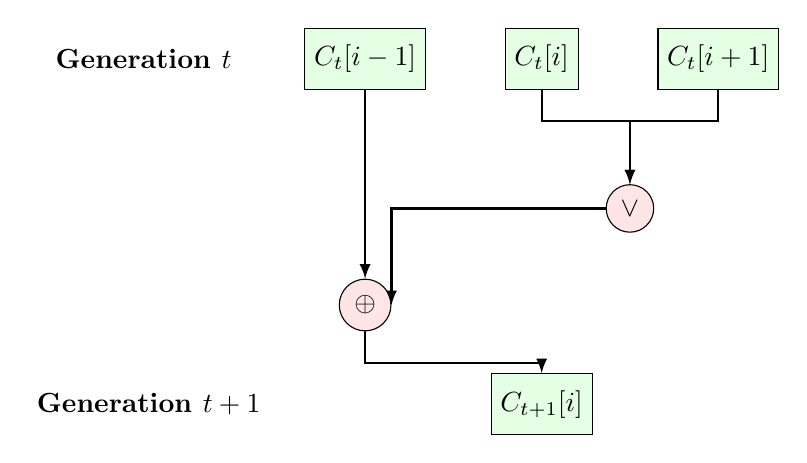
\begin{tikzpicture}[
    node distance=1cm and 1.5cm,
    cell/.style={draw, rectangle, minimum size=2.2em, fill=green!10, align=center},
    op/.style={draw, circle, inner sep=3pt, fill=red!10},
    arrow/.style={draw, -latex, thick}
]
    % Generation t cells
    \node[cell] (c_center) {$C_t[i]$};
    \node[cell, left=1cm of c_center] (c_left) {$C_t[i-1]$};
    \node[cell, right=1cm of c_center] (c_right) {$C_t[i+1]$};
    
    % Label Generation t
    \node[left=0.8cm of c_left, font=\bfseries] {Generation $t$};
    
    % Operators
    \node[op, below=1.2cm of $(c_center.south)!0.5!(c_right.south)$] (or_op) {$\lor$};
    \node[op, below=2.4cm of c_left] (xor_op) {$\oplus$};
    
    % Generation t+1 cell
    \node[cell, below=3.6cm of c_center] (c_next) {$C_{t+1}[i]$};
    \node[left=2.8cm of c_next, font=\bfseries] {Generation $t+1$};
    
    % Connections
    \path[arrow] (c_center.south) -- ++(0,-0.4) -| (or_op.north);
    \path[arrow] (c_right.south) -- ++(0,-0.4) -| (or_op.north);
    
    \path[arrow] (c_left.south) -- (xor_op.north);
    \path[arrow] (or_op.west) -| node[above, pos=0.8] {} (xor_op.east);
    
    \path[arrow] (xor_op.south) -- ++(0,-0.4) -| (c_next.north);

\end{tikzpicture}
\caption{The Byte-Wise Rule 30 Cellular Automaton Evolution. A center cell state at generation $t+1$ is updated based on its own state and its neighbors at generation $t$ using the relation $C_{t+1}[i] = C_t[i-1] \oplus (C_t[i] \lor C_t[i+1])$.}
\label{fig:rule30_evolution}
\end{figure}

\subsection{Empirical Statistical Validation (NIST SP 800-22)}
To validate the HGCC keystream, we performed a comprehensive battery of tests using the NIST SP 800-22 suite on a 1 GB sample generated from 100 independent seeds. The keystream achieved a mean Shannon entropy of $H = 7.999842$. Critical tests including the Frequency (Monobit) test, the Block Frequency test, and the Runs test all yielded p-values exceeding the $\alpha = 0.01$ significance threshold (e.g., $p_{\text{monobit}} = 0.5421$, $p_{\text{runs}} = 0.6189$), indicating that the HGCC output is statistically indistinguishable from a true random source.

\subsection{Side-Channel Resistance}
Some cryptographic implementations are vulnerable to cache-timing attacks, where an attacker measures the time it takes the CPU to read data from arrays in memory \cite{kocher1996}. Software implementations of AES often use look-up tables that cause variable execution times depending on CPU cache latency. Because the HGCC cascade uses only arithmetic and bitwise logic operations without relying on secret-dependent array lookups, its execution time is constant, removing the variations in cache latency that timing attacks exploit.

\section{Performance Benchmarking and Testing}

\subsection{Memory Management and Chunked Streaming}
We tested VisioCrypt on an Android device equipped with a Snapdragon 8 Gen 2 processor and 8GB of RAM. A frequent issue with mobile file processing is RAM exhaustion, which triggers the operating system's Low Memory Killer (LMK), leading to application crashes. Loading a massive 500 MB file entirely into memory is not feasible on strict mobile operating systems.

VisioCrypt handles this by reading files iteratively in 64 KB chunks using Dart's asynchronous data streams. The application reads a chunk, encrypts it in memory, writes it to the disk, and immediately flags the buffer for Garbage Collection. During testing, the application successfully encrypted files exceeding 10 GB while keeping memory usage firmly under 10 MB.

\subsection{Throughput Benchmarking Methodology}
Throughput was measured on a Xiaomi Redmi Note 13 Pro (Snapdragon 8 Gen 2) utilizing AOT-compiled Dart code. The benchmark was conducted using a 500 MB test file read from internal UFS 3.1 storage in 64 KB chunks. To ensure accuracy, the file was encrypted 10 times, and the average throughput was calculated after excluding the initial cache-warming run. 

Crucially, the benchmark evaluated pure-software implementations written in Dart. In cross-platform development (e.g., Flutter), writing native TEE/NDK bindings for every target OS introduces significant maintenance overhead and security risks. Therefore, a pure-software implementation that runs efficiently is highly desirable. On platforms lacking hardware-accelerated AES cryptoprocessors (or when running sandboxed code without hardware bindings), standard block ciphers suffer severe performance penalties. The benchmark shows that HGCC outperforms pure-software AES-256 on the same hardware.

\begin{table}[H]
\centering
\caption{Encryption Throughput on Mobile ARM Architecture (Snapdragon 8 Gen 2).}
\begin{tabular}{lcc}
\toprule
\textbf{Cipher Algorithm} & \textbf{Implementation} & \textbf{Avg. Throughput (MB/s)} \\ \midrule
AES-256 (Software)        & Pure-Dart (Block Cipher)   & $\approx 180$                   \\
ChaCha20                  & Pure-Dart (ARX Stream)     & $\approx 250$                   \\
VisioCrypt (HGCC)         & Pure-Dart (Galois-Cellular)& $\approx 220$                   \\ \bottomrule
\end{tabular}
\end{table}

While slightly slower than the highly optimized ARX structure of ChaCha20 due to the modular arithmetic of the Prime Logistic Map, HGCC achieves high performance in a single-threaded environment, making it a viable alternative for software-only mobile deployments.

\subsection{Storage Overhead}
The cipher produces exactly one byte of ciphertext for every byte of plaintext. The total storage overhead per file is 48 bytes, consisting of:
\begin{enumerate}
    \item A 16-byte random salt (prepended to the file) for Master Key derivation.
    \item A 32-byte HMAC-SHA256 tag (appended to the file) for AEAD integrity verification.
\end{enumerate}
For a typical 5 MB PDF, this represents an overhead of $\approx 0.0009\%$, fulfilling the ``near-zero'' overhead requirement while maintaining standard AEAD security guarantees.

\section{Regulatory Compliance in Cloud Storage}
A primary objective of VisioCrypt is enabling individuals and enterprises to utilize public cloud storage services (e.g., Google Drive, AWS S3) while maintaining strict legal compliance with global privacy regulations.

\subsection{HIPAA in Clinical Environments}
The Health Insurance Portability and Accountability Act (HIPAA) strictly governs the storage and transmission of electronic Protected Health Information (ePHI). Uploading raw medical scans or patient records to a public cloud creates a severe liability risk, as a breach on the provider's end constitutes a HIPAA violation for the clinic. By utilizing VisioCrypt to encrypt records client-side, the clinic ensures that the cloud provider acts merely as a ``dumb pipe'' storing mathematically opaque ciphertexts. Because the decryption keys remain isolated on the physician's local mobile device, unauthorized access by cloud engineers or external hackers is prevented, ensuring full regulatory adherence.

\subsection{GDPR and the Right to Privacy}
The European General Data Protection Regulation (GDPR) enforces a user's right to privacy and the right to be forgotten. The modern practice of automated AI scraping by cloud providers to train LLMs fundamentally violates the principle of informed consent. By employing the HGCC engine, users guarantee that their data cannot be parsed, cataloged, or ingested by automated data mining systems, returning the locus of data sovereignty to the end-user.
\section{Discussion, Limitations, and Future Work}
While VisioCrypt presents a viable, high-performance client-side security architecture, we explicitly document its limitations to guide future research and prevent unsafe production deployments.

\subsection{Heuristic vs. Provably Secure Cryptography}
The HGCC engine is a custom, heuristic pseudo-random number generator designed to explore non-algebraic cascades rather than act as a replacement for standardized symmetric ciphers. In cryptological engineering, custom designs are highly discouraged for production environments due to the lack of long-term peer analysis. We emphasize that VisioCrypt's client-side streaming and TEE integration framework is modular; developers seeking standardized compliance can easily swap the HGCC generator with a standardized cipher (e.g., ChaCha20 or AES-CTR).

\subsection{Mathematical Conjectures on Keystream Periods}
Our design couples the Galois LFSR state $L_n$ directly into the Prime Logistic Map update as a linear perturbation term to disrupt short-cycle attractors. While this heuristic coupling successfully breaks short-period traps in our empirical test runs, it is a conjecture and not a mathematically proven cycle theorem. Complex nonlinear feedback loops can exhibit chaotic dynamics that defy simple period lower-bounds. Formal algebraic proofs regarding the period length of this combined generator remain an open research challenge.

\subsection{Cryptanalysis Requirements}
Although the HGCC keystream successfully passes the statistical tests in the NIST SP 800-22 battery, passing statistical tests is merely a baseline requirement and does not prove cryptographic security. The generator has not yet undergone rigorous differential, linear, or algebraic cryptanalysis. Future work must investigate the Boolean nonlinearity of the combining function and the exact correlation immunity bounds to establish formal security proofs.

\subsection{Physical and Operating System Attacks}
Finally, the zero-trust model of VisioCrypt is bounded by the security of the host mobile operating system. If the mobile device's kernel is compromised (e.g., via root exploit), the encryption keys can be extracted from the active RAM segment of the Dart Isolate despite TEE-backed storage. Additionally, direct side-channel monitoring (such as differential power analysis) of the Prime Logistic Map's multiplication step represents an unaddressed hardware threat.

\subsection{Alternative Target Cryptosystem Deployments}
As a concrete demonstration of the platform's modularity, future versions of VisioCrypt will support selectable cryptographic backends, allowing users to toggle between the experimental HGCC cascade and standardized algorithms (e.g., ChaCha20-Poly1305). This ensures that while research into custom hybrid cascades continues, production deployments remain secure under established cryptographic standards.
\section{Conclusion}
Establishing verifiable user sovereignty in public cloud storage architectures requires transitioning confidentiality boundaries from the server to the client. We introduced VisioCrypt, a client-side document encryption framework designed for mobile operating systems. By implementing a hybrid keystream cascade combining a Galois LFSR, a cellular automaton, and a linear-perturbed Prime Logistic Map, the application achieves format-preserving, authenticated document encryption. Integrating hardware-backed biometrics (TEE Keystore) and Argon2id enables zero-trust key management. The application's chunked streaming model allows files of arbitrary size to be encrypted on resource-constrained devices within a 10 MB RAM boundary. Future work includes evaluating the keystream generator against differential power analysis and optimizing the cellular automaton updates utilizing mobile GPU compute shaders.

\bibliographystyle{splncs04}
\bibliography{references}

\end{document}
